\documentclass[conference,10pt]{IEEEtran}
\usepackage[T1]{fontenc}
\usepackage{microtype}
\usepackage{booktabs}
\usepackage{tikz}
\usetikzlibrary{arrows.meta,positioning,fit}
\usepackage{xurl}
\usepackage[hidelinks]{hyperref}
\usepackage{cite}

\newcommand{\sh}{\textsc{SpecHunter}}

\begin{document}

\title{\sh{}: A Fail-Closed Agent Loop for Security Discovery and Repair on BOOM RTL}

\author{\IEEEauthorblockN{Ariel Khais \quad Ryan Chen \quad Cambell Xiao}
\IEEEauthorblockA{University of Washington\\
\{akhais, ryanc175, cambell\}@uw.edu}}

\maketitle

\begin{abstract}
We present \sh{}, a CHIA loop in which LLM agents propose attack programs,
repairs, and follow-up attacks against the BOOM out-of-order RISC-V core, while a
deterministic validator decides every verdict from cycle-accurate simulation.
The design premise is that an agent's claims are cheap and its mistakes are
plausible, so the loop's value lies in what it refuses to accept. In a live run,
Gemini~2.5 Flash-Lite drove the loop against a Verilator build of SmallBoomV3:
it found an intentionally seeded cache leak, minimized it to a three-operation
witness, selected a repair, and the validator required a clean retest and
attacker exhaustion before accepting it (28 BOOM executions, 4 model calls,
\$0.0006). An eight-program held-out corpus then separated the vulnerable and
repaired variants in all 64 executions. We also applied the loop to upstream
BOOM issue~\#715 on the exact reported revision. The waveform trace shows that
the address first taken as evidence of leakage comes from an unrelated
load, while the dependent load is stopped by an existing register-read gate. As
a result, the issue did not reproduce, and none of four candidate RTL repairs can be
credited. We report these negative results and eleven verifier defects exposed by
live runs and their review, because they are the part of this work most likely to be
useful to others building agentic hardware-security loops.
\end{abstract}

\section{Introduction}
Transient-execution attacks~\cite{spectre,meltdown} arise from interactions
between speculation, privilege checks, and cache state that are hard to
enumerate by hand. LLM agents can write plausible attack programs and RTL
patches quickly, which makes them attractive for security red-teaming of
open cores. They are also very good at producing \emph{plausible but wrong}
conclusions: a repair that ``fixes'' a leak that never occurred, a minimized
witness that no longer exercises the threat, or a clean retest that is clean
because the attack became irrelevant. In hardware security these mistakes are
expensive: a single simulator run of an out-of-order core takes seconds to
minutes, and a false ``fixed'' verdict can send a design team chasing a bug that
was never there.

\sh{} is a CHIA~\cite{chia} loop for the BOOM core~\cite{boom} in
Chipyard~\cite{chipyard}, built around one rule: \emph{agents propose, the
validator disposes}. Agents never emit executable patches or observations;
they select from closed, reviewed program operations and repair identifiers,
and every verdict is recomputed from raw simulator output bound by SHA-256 to
the exact source, binary, and runner that produced it. The loop is deliberately
conservative: any result that is not a deterministic, secret-dependent,
architecturally silent leak is treated as inconclusive rather than clean, so the
loop fails closed. Our contributions are:
\begin{itemize}
\item A four-agent CHIA loop (recon, attacker, validator, repair) with
  mandatory witness retest and a strict attacker-exhaustion criterion, running
  against cycle-accurate BOOM with Spike~\cite{spike} as the architectural
  reference and an atomic cost ledger (\S\ref{sec:loop}).
\item End-to-end evidence on real BOOM RTL, clearly separated from fixture and
  model-only evidence, with every number bound into a recomputable seal
  (\S\ref{sec:eval}).
\item A trace-level investigation of BOOM issue~\#715~\cite{issue715} on its
  historical revision that did \emph{not} reproduce the reported mechanism and
  identified why (\S\ref{sec:715}).
\item A catalogue of verifier defects found during live runs, each now
  covered by a regression test (\S\ref{sec:lessons}).
\end{itemize}

\section{Loop Design}\label{sec:loop}
\begin{figure}[t]
\centering
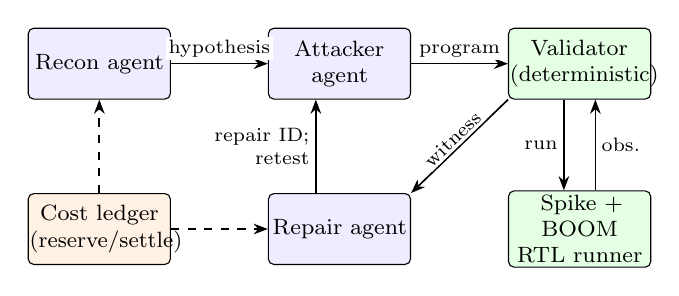
\begin{tikzpicture}[
  box/.style={draw,rounded corners=2pt,align=center,font=\footnotesize,minimum height=9mm,text width=17mm,inner sep=1.5pt},
  agent/.style={box,fill=blue!7},
  trusted/.style={box,fill=green!10},
  lbl/.style={font=\scriptsize,fill=white,inner sep=1pt},
  arr/.style={-{Stealth[length=1.8mm]},semithick}]
\node[agent] (recon) at (0,0) {Recon agent};
\node[agent] (atk) at (3.05,0) {Attacker agent};
\node[trusted] (val) at (6.1,0) {Validator\\(deterministic)};
\node[box,fill=orange!10] (led) at (0,-2.1) {Cost ledger\\(reserve/settle)};
\node[agent] (rep) at (3.05,-2.1) {Repair agent};
\node[trusted] (sim) at (6.1,-2.1) {Spike + BOOM\\RTL runner};
\draw[arr] (recon) -- node[lbl,above=1pt]{hypothesis} (atk);
\draw[arr] (atk) -- node[lbl,above=1pt]{program} (val);
\draw[arr] ([xshift=-2mm]val.south) -- node[lbl,left=1pt]{run} ([xshift=-2mm]sim.north);
\draw[arr] ([xshift=2mm]sim.north) -- node[lbl,right=1pt]{obs.} ([xshift=2mm]val.south);
\draw[arr] (val.south west) -- node[lbl,sloped,above=0pt]{witness} (rep.north east);
\draw[arr] ([xshift=-3mm]rep.north) -- node[lbl,left=1pt,align=right]{repair ID;\\retest} ([xshift=-3mm]atk.south);
\draw[arr,dashed] (led) -- (recon);
\draw[arr,dashed] (led) -- (rep);
\end{tikzpicture}
\caption{The \sh{} loop. Blue: LLM agents (Gemini 2.5 Flash-Lite via Vertex
AI). Green: trusted, deterministic components that decide every verdict.}
\label{fig:loop}
\end{figure}

\textbf{Agents.} Figure~\ref{fig:loop} shows the loop. The recon agent states
a hypothesis against a security invariant (user code must not observe a
PMP-protected secret, architecturally or through cache timing). The attacker
turns it into a program over a whitelist of operations (e.g.,
\texttt{enter\_user}, \texttt{train\_branch}, \texttt{load\_secret},
\texttt{encode}, \texttt{probe}); the trusted runner compiles these to fixed,
reviewed RV64 instruction templates. The repair agent may only choose a
closed repair ID; it cannot emit patch text. This closed interface is what lets
an untrusted model drive a privileged experiment: the agent chooses \emph{which}
reviewed building blocks to combine, never the machine code that runs.

\textbf{Threat model and harness.} The invariant is user/supervisor isolation:
code in user mode must not learn a byte of a PMP-protected supervisor page, either
architecturally or through a timing side channel. The reviewed harness builds on
the RISC-V test/HTIF substrate. It reserves an aligned 4\,KiB secret page,
configures PMP to deny it, installs a machine-mode trap handler, and enters user
mode with \texttt{mret}. A denied load and its dependent encode/squash window are
skipped architecturally after the load-access fault (cause~5); a fixed probe then
times the same two public cache lines in the same order and reports only whether
line~0 was faster. Neither the probe addresses nor its control flow depend on the
secret, so the probe itself cannot manufacture a signal. Spike and BOOM must
agree on architectural output and trap events before a BOOM observation is
accepted; any disagreement, unexpected trap, or timeout is inconclusive.

\textbf{Validator.} Each candidate runs in four executions: two secret values,
each repeated twice. A violation requires a deterministic, secret-dependent
observation with the expected load-access fault and no architectural secret
value; anything else is \emph{inconclusive}, never clean. Findings are
minimized by delta debugging, and the minimized program must itself reproduce
before it is recorded.

\textbf{Repair acceptance.} After a repair, the orchestrator (not the model)
replays the exact minimized witness, which must be clean. Control then returns
to the attacker. A repair is verified only on attacker exhaustion, and in
the current schema (v5) exhaustion additionally requires a distinct,
threat-relevant challenge that violates on the \emph{unrepaired} variant and is
clean on the repaired one. Any later violation revokes verification.

\textbf{Provenance and cost.} Chipyard 1.14, BOOM, and toolchains are pinned by
commit and hash; the runner refuses dirty trees or mismatched binaries. Every
evidence file is bound into a SHA-256 seal, and a single verifier recomputes all
43 file bindings across the ten seals and rebuilds the issue~\#715 case seal from
its raw waveforms; continuous integration runs it on every change. A locked JSON
ledger reserves a conservative cost before each model call and settles it from
token metadata, halting at a hard cap. \sh{} runs as a decorated CHIA node on a
local Ray runtime.

\section{Evaluation}\label{sec:eval}
All BOOM runs used GCP \texttt{e2-standard-8} workers with no service account,
a six-hour deletion cap, and explicit deletion after evidence recovery.
Table~\ref{tab:evidence} lists every result together with the kind of
target it was measured on; we do not combine results across kinds.

\begin{table}[t]
\centering
\caption{Sealed evidence by target type. ``Mutation'' is an intentionally
seeded harness leak, not an upstream BOOM bug.}
\label{tab:evidence}
\footnotesize
\setlength{\tabcolsep}{3pt}
\begin{tabular}{@{}p{0.40\columnwidth}p{0.25\columnwidth}p{0.29\columnwidth}@{}}
\toprule
Experiment & Target & Result \\
\midrule
PMP privilege gate (Spike + BOOM) & BOOM RTL & pass, trap 5, no leak \\
Pristine baseline matrix & BOOM RTL & 8/8 clean \\
Seeded positive control & BOOM+mutation & 8/8 violating; 8/8 clean after repair \\
Live Vertex loop & BOOM+mutation & found, repaired, exhausted; \$0.0006 \\
Held-out corpus (8 programs) & BOOM+mutation & 64/64 correct \\
LSU fault-gate RTL patch & patched BOOM & builds; 8/8 clean; \emph{no security claim} \\
Issue \#715, current + historical & BOOM RTL & not reproduced \\
Guided vs.\ random search & Fixture & see Table~\ref{tab:search} \\
10$\times$ loop repeatability & Model fixture & 10/10; \$0.0054 total \\
Loop through CHIA node & Model fixture & complete; \$0.0005 \\
\bottomrule
\end{tabular}
\end{table}

\textbf{Real BOOM baseline.} A reviewed payload configures PMP to deny a
4\,KiB page, drops to user mode via \texttt{mret}, and requires a
load-access fault (cause~5). The same ELF passed on Spike and on SmallBoomV3.
Two programs (architectural denial and a transient window) were clean and
deterministic across secret worlds on the pristine core. Because pristine BOOM
exhibited no violation, we added a clearly labelled positive control: a
harness variant that touches a secret-selected cache line before entering user
mode. Its repair, \texttt{remove-seeded-cache-leak}, removes that access. The
control produced probe sequences \texttt{[1],[0],[1],[0]} before repair and
all zeros after, over 16 executions on the \emph{same} simulator binary.

\textbf{Live agent run.} On the positive control, the model proposed a
six-operation program; BOOM confirmed the leak; minimization kept
\texttt{enter\_user, load\_secret, probe}. The repair agent chose the
closed repair, the witness retested clean, and the attacker then reached
exhaustion: 28 BOOM executions, 4 Vertex calls, zero inconclusive cases, and
\$0.0006038 of accounted cost. This transcript predates the schema-v5
exhaustion rule and exhausted after only the mandatory replay; under the
current rule it would require one further discriminating challenge.

\textbf{Held-out corpus.} Eight fixed programs vary training, encoding,
squash and fence placement, and noise, all retaining the protected load. With
two repetitions in both secret worlds, all 32 mutated executions were
deterministic violations and all 32 repaired executions were clean. This
tests that the \emph{validator and repair gate} generalize across program
shape; it does not test an RTL fix.

\textbf{Candidate RTL patch.} Source review of BOOM's \texttt{lsu.scala} found
that incoming and retried D-cache requests are not gated by same-cycle
\texttt{ae\_ld}/\texttt{pf\_ld}/\texttt{ma\_ld}. A two-path gate patch built
into a distinct simulator and ran the secure matrix cleanly (8/8). Since the
baseline was already clean, this shows only that the patch builds and does not
break the target tests. The seal records \texttt{security\_fix\_validated:
false}.

\begin{table}[t]
\centering
\caption{Search on deterministic fixtures (privilege, transient-cache, and
secure-control benchmarks; 16-iteration budget).}
\label{tab:search}
\footnotesize
\begin{tabular}{@{}lcc@{}}
\toprule
 & Guided & Random (1000 seeds) \\
\midrule
Positive cases found & 2/2 & 1145/2000 (57.3\%) \\
95\% Wilson interval & -- & 55.1--59.4\% \\
Mean attempts to find & 1.5 & 8.48 \\
False positives (secure control) & 0 & 0/1000 \\
\bottomrule
\end{tabular}
\end{table}

\textbf{Search and repeatability.} Table~\ref{tab:search} compares the
deterministic guided policy with random programs over three small fixtures.
The guided arm is a single deterministic run, so this is a sanity check on
search structure, not a statistical claim about LLM agents. Separately, ten
independent Gemini-driven trials on a fast model of the positive control all
completed discovery, repair, retest, and exhaustion (40 calls, 264 fixture
executions, \$0.0053752). A further run through the CHIA
\texttt{run\_agent\_experiment} node (CHIA 1.0.1, Ray 2.54.0) completed the
same lifecycle for \$0.0005130.

\section{Case Study: BOOM Issue \#715}\label{sec:715}
Issue~\#715~\cite{issue715} reports that on a historical BOOM a
supervisor-page load that faults can still forward data to a dependent load
during speculation, leaking it through the TLB. We tested it three ways.

\textbf{Adaptation.} A reviewed adaptation of the mechanism was deterministic and
clean on the current pin (4 executions) and on the exact reported
Chipyard \texttt{004297b6}/BOOM \texttt{fac2c370} with historical
\texttt{SmallBoomConfig} (built in 685\,s).

\textbf{Original attachment.} We fetched the reporter's ELF by pinned URL and
digest, converted its entry-zero image to a fixed load image, and captured a
VCD waveform at a fixed seed. Table~\ref{tab:gadget} summarizes the gadget. A scanner joins events by ROB index,
physical register, load-queue slot, and branch mask, and requires one ordered
chain within the first speculation window. The trace shows the trained branch
(cycle 3769), a branch-masked protected-page TLB request (3807), requests to
\texttt{0x59f} (from 3809), a page fault, and misprediction resolution (3910).
At first sight this looks like the reported leak. However, the disassembly shows that
\texttt{0x59f} is the address of an independent third load
(\texttt{lb s1, 1439(a0)} with a zero base; $1439 = \texttt{0x59f}$), not a
secret-derived address. The dependent load at gadget offset +4 issues with its source operand
poisoned while the LSU reports a load miss, and BOOM's register-read gate
(\texttt{exu/core.scala}, lines 973--978) drops its issue-valid, so it never
presents a valid LSU request.

\begin{table}[t]
\centering
\caption{Issue \#715 attachment gadget (wrong path) and what the
historical-RTL waveform shows for each load.}
\label{tab:gadget}
\footnotesize
\setlength{\tabcolsep}{3pt}
\begin{tabular}{@{}lll@{}}
\toprule
Offset & Instruction & Observed in waveform \\
\midrule
+0 & \texttt{lb sp,-2048(t1)} & protected-page TLB req.\ (3807); fault \\
+4 & \texttt{ld s1,0(sp)} & issues poisoned; register read gated \\
+8 & \texttt{lb s1,1439(a0)} & requests \texttt{0x59f} (from 3809) \\
\bottomrule
\end{tabular}
\end{table}

\textbf{Repairs.} Before this attribution was clear, we iterated on four
hash-pinned candidate LSU patches outside the closed repair list, each driven
by the previous matched-trace comparison: v1 same-cycle fault gates; v2 blocking loads
under unresolved branches; v3 suppressing fast wakeup and excepting-entry
writeback; v4 requiring a registered D-cache fire before speculative wakeup.
V1--v3 left the \texttt{0x59f} chain cycle-identical to baseline, and v4's
waveform was not recovered. Because the baseline never demonstrated the
dependent-load mechanism, \emph{no} repair can be credited, and every
comparison seal records \texttt{security\_fix\_validated: false}.
A loop that accepted ``the patch built and nothing leaked'' would have
declared success four times here.

\section{What the Live Runs Taught Us}\label{sec:lessons}
Table~\ref{tab:lessons} lists verifier defects exposed by live runs or
review of their transcripts. Each would have produced an unsupported claim.
Each is now covered by a regression test.

\begin{table}[t]
\centering
\caption{Verifier defects found and closed. FP = would have enabled a false
positive (a false finding or false ``fixed'').}
\label{tab:lessons}
\footnotesize
\setlength{\tabcolsep}{3pt}
\begin{tabular}{@{}p{0.72\columnwidth}p{0.2\columnwidth}@{}}
\toprule
Defect & Effect \\
\midrule
Minimizer could drop the protected load from a witness & FP finding \\
Retest of the same program counted toward exhaustion & FP fix \\
Irrelevant (e.g.\ probe-only) challenge counted as clean & FP fix \\
Challenge clean on \emph{both} variants counted as clean & FP fix \\
Verified flag survived a later-cycle violation & FP fix \\
Stale clean-replay flag carried across recon cycles & FP fix \\
Short observation batch skipped repeatability check & FP either \\
VCD scanner read intermediate combinational values & FP finding \\
Unrelated trace events could form a ``mechanism chain'' & FP finding \\
Seed equality inferred from matching timing & provenance \\
Git porcelain \texttt{.strip()} rejected valid repair tree & false reject \\
\bottomrule
\end{tabular}
\end{table}

Three lessons generalize. First, \emph{a clean result is only evidence if the
same test fails on the vulnerable variant}; four of the defects are versions
of this. Second, minimizers and scanners are adversarial surfaces: they
optimize for the property check, not the threat model, and must re-encode the
threat model as constraints. Third, a negative result on real RTL (issue~\#715)
required more infrastructure than the positive control, and it is also the
more informative of the two.

\section{Related Work}\label{sec:related}
Hardware fuzzing drives RTL toward coverage without a security oracle:
RFUZZ~\cite{rfuzz} mutates inputs to maximise mux-toggle coverage on FPGAs.
Security-oriented differential fuzzing adds an oracle by comparing a design
against a reference or against itself under different secrets, the strategy our
validator follows for BOOM. Hardware--software contracts~\cite{contracts} give a
formal specification for what speculation may and may not expose, and are a
natural target invariant for a future version of \sh{}. Relative to this line of
work, \sh{} contributes the agentic control loop and, more importantly, a
fail-closed evidence discipline: an untrusted model may steer the search, but no
claim survives that a deterministic oracle and a recomputable seal do not
independently support.

\section{Limitations and Future Work}\label{sec:limits}
We found no new BOOM vulnerability; every successful discovery and repair is on an
intentional harness mutation. The live BOOM loop ran once; repeatability is
shown on a model fixture only. The search comparison uses three small fixtures.
Repairs are chosen from a closed list, so the agent diagnoses rather than
synthesizes RTL, a deliberate trade of generality for soundness. The cache
observer covers two lines in a fixed order. The clearest next step that keeps the
soundness guarantees is to widen the attacker's parameterized primitives and the
observation channel while holding the differential oracle fixed, and to target a
\emph{published} transient-execution class as a reproduction before attempting
anything novel; the oracle, not the model, would still decide every verdict.

\section{Conclusion}
\sh{} shows that an LLM-driven security loop on real out-of-order RTL is cheap
to run (under a tenth of a cent per live cycle) and that its credibility comes
from a validator that fails closed. The loop, pinned BOOM runners, and every
sealed artifact are open source at
\url{https://github.com/Ryclic/SpecHunter}.

\section*{AI Assistance Disclosure}
Gemini 2.5 Flash-Lite is a component of the evaluated loop. AI coding
assistants (OpenAI Codex, Google Gemini/Antigravity, and Anthropic Claude Code)
were used to write and review code and tests, analyze evidence, and draft and
edit this paper. The human authors reviewed all claims against the sealed
evidence and are responsible for the paper's content.

\bibliographystyle{IEEEtran}
\bibliography{main}

\end{document}
